\documentclass[ncrna,article,submit,moreauthors,pdftex,10pt,a4paper]{mdpi} 
\usepackage{color}
\usepackage{subfigure}
\newcommand{\TODO}[1]{\begingroup\color{red}#1\endgroup}
\newcommand{\update}[1]{\begingroup\color{blue}#1\endgroup}
%=================================================================
\firstpage{1} 
\makeatletter 
\setcounter{page}{\@firstpage} 
\makeatother 
\articlenumber{x}
\doinum{10.3390/------}
\pubvolume{xx}
\pubyear{2016}
\copyrightyear{2016}
\externaleditor{Academic Editor: name}
\history{Received: date; Accepted: date; Published: date}
\history{ }
%=================================================================
\Title{Rare Splice Variants in Long Non-Coding RNAs}

\Author{Rituparno Sen$^{1}$, Gero Doose$^{2}$, 
   Peter F. Stadler$^{2-8}$*}

% Authors, for metadata in PDF
\AuthorNames{Rituparno Sen, Gero Doose, Peter F. Stadler}

\address{%
  $^{1}$Bioinformatics Group, Dept.\ Computer Science, and
  Interdisciplinary Center for Bioinformatics, University Leipzig,
  H{\"a}rtelstrasse 16-18, D-04107 Leipzig, Germany\\
  $^{2}$ecSeq Bioinformatics, Brandvorwerkstra{\ss}e 43,
  D-04275 Leipzig, Germany\\
  $^{3}$German Centre for Integrative Biodiversity Research (iDiv)
  Halle-Jena-Leipzig, Competence Center for Scalable Data Services and
  Solutions; Leipzig Research Center for Civilization Diseases; and Leipzig
  Research Center for Civilization Diseases (LIFE), University Leipzig\\
  $^{4}$Max Planck Institute for Mathematics in the Sciences,
  Inselstra{\ss}e 22, D-04103 Leipzig, Germany\\
  $^{5}$Fraunhofer Institute for Cell Therapy and Immunology,
  Perlickstrasse 1, D-04103 Leipzig, Germany\\
  $^{6}$Center for RNA in Technology and Health, Univ. Copenhagen,
  Gr{\o}nneg{\aa}rdsvej 3, Frederiksberg C, Denmark\\
  $^{7}$Santa Fe Institute, 1399 Hyde Park Road, Santa Fe NM 87501, USA }

\corres{Correspondence: studla@bioinf.uni-leipzig.de; Tel.: +49 341 97-16690}

\abstract{Long noncoding RNAs(lncRNAs) are constantly being discovered and
  we are in a nascent stage of understanding their sequence structure. We
  performed statistical analyses on exon and intron content of lncRNA
  annotation data from different publicly available annotation datasets.
  We have used sophisticated alignment algorithms as well as custom
  analysis scripts to investigate the transcriptomic structure of lncRNAs.}

\keyword{lncRNA, splice junctions, GENCODE, lncRNA isoforms}

\begin{document}

\section{Introduction}

Long non-coding RNAs (lncRNAs) are an important part of the mammalian
transcriptome \cite{Clark:11a,ENCODE:12}. Although the set of lncRNAs that
is well understood with respect to biological function and molecular
mechanism is still limited, it is rapidly expanding. Genes such as ANRIL
\cite{Li:16A,Aguilo:16}, HULC \cite{Yu:17}, MALAT1 \cite{Liu:17}, TUG1
\cite{Li:16}, or Xist \cite{daRocha:17} may serve as examples. Wide-spread
roles include, but are not limited to, interactions with chromatin to
silence or activate chromatin \cite{guttmannat2012,Deng:16} and the
regulation of splicing \cite{Luco:16}. Still the coverage and precision of
the lncRNA annotation lack behind the accurate maps of protein-coding
genes.  The GENCODE project \cite{harrow2012} provides the most accurate
transcript and gene annotation for the human genome. It is a combination of
manual and automated annotation techniques which endeavours to list gene
features from HAVANA and Ensembl datasets. Detailed surveys of expression
patterns across many tissue and cell-types, see e.g.\
\cite{cabili2011,MasPonte:17,Hon:17} provide evidence for intricate
regulatory networks in which lncRNAs key players.

There is mounting evidence, however, that lncRNA isoforms may differ
drastically in their biological function \cite{Holdt:13a,Bozgeyik:16}. Due
to their usally low expression values, gene models for lncRNAs historically
were often truncated, a situation that only has been improving recently.
Notably, the recent lncRNA atlas by Hon \emph{et al.} \cite{Hon:17}
specifically aimed at providing accurate 5' ends. The situation is still
more difficult at the 3' side, since long, large unspliced 3' regions make
it difficult determine complete transcript from Illumina data, see e.g.\
\cite{Mercer:10,Engelhardt:15a}. Furthermore, lncRNAs such as ANRIL
\cite{Holdt:13a}, exhibit complex patterns of alternative splicing. Even in
extremely well-studied protein-coding loci, rare isoforms keep being
discovered \cite{Hoffmann:14a}. It thus remains an unresolved question to
what extent the current maps of lncRNAs are complete both in terms of the
number of expressed loci/gene and in terms of the variability of their
isoforms. 

One component towards answering this question is to ask to what extent the
transcript portfolio of a particular cell type has been mapped completely.
Conversely, one asks in this context to what extent reported transcripts are
noise. To address these issues we investigate here a very large set of
transcriptome data from B cell lymphomas. By virtue of aggregating hundreds
of independently generated transcriptome data set we can study in detail if
and the set of detectable splice junctions converges to a consensus.

\section{Results}

Fig.~\ref{fig:saturation} summarize the effect of increasing coverage on
the estimated average number of introns per gene locus. The data
qualitatively reproduce that observation of the ENCODE project that there is
a large difference in the average number of splice junctions between
protein-coding loci and ncRNAs. 

\begin{figure}[t]
\begin{center}
  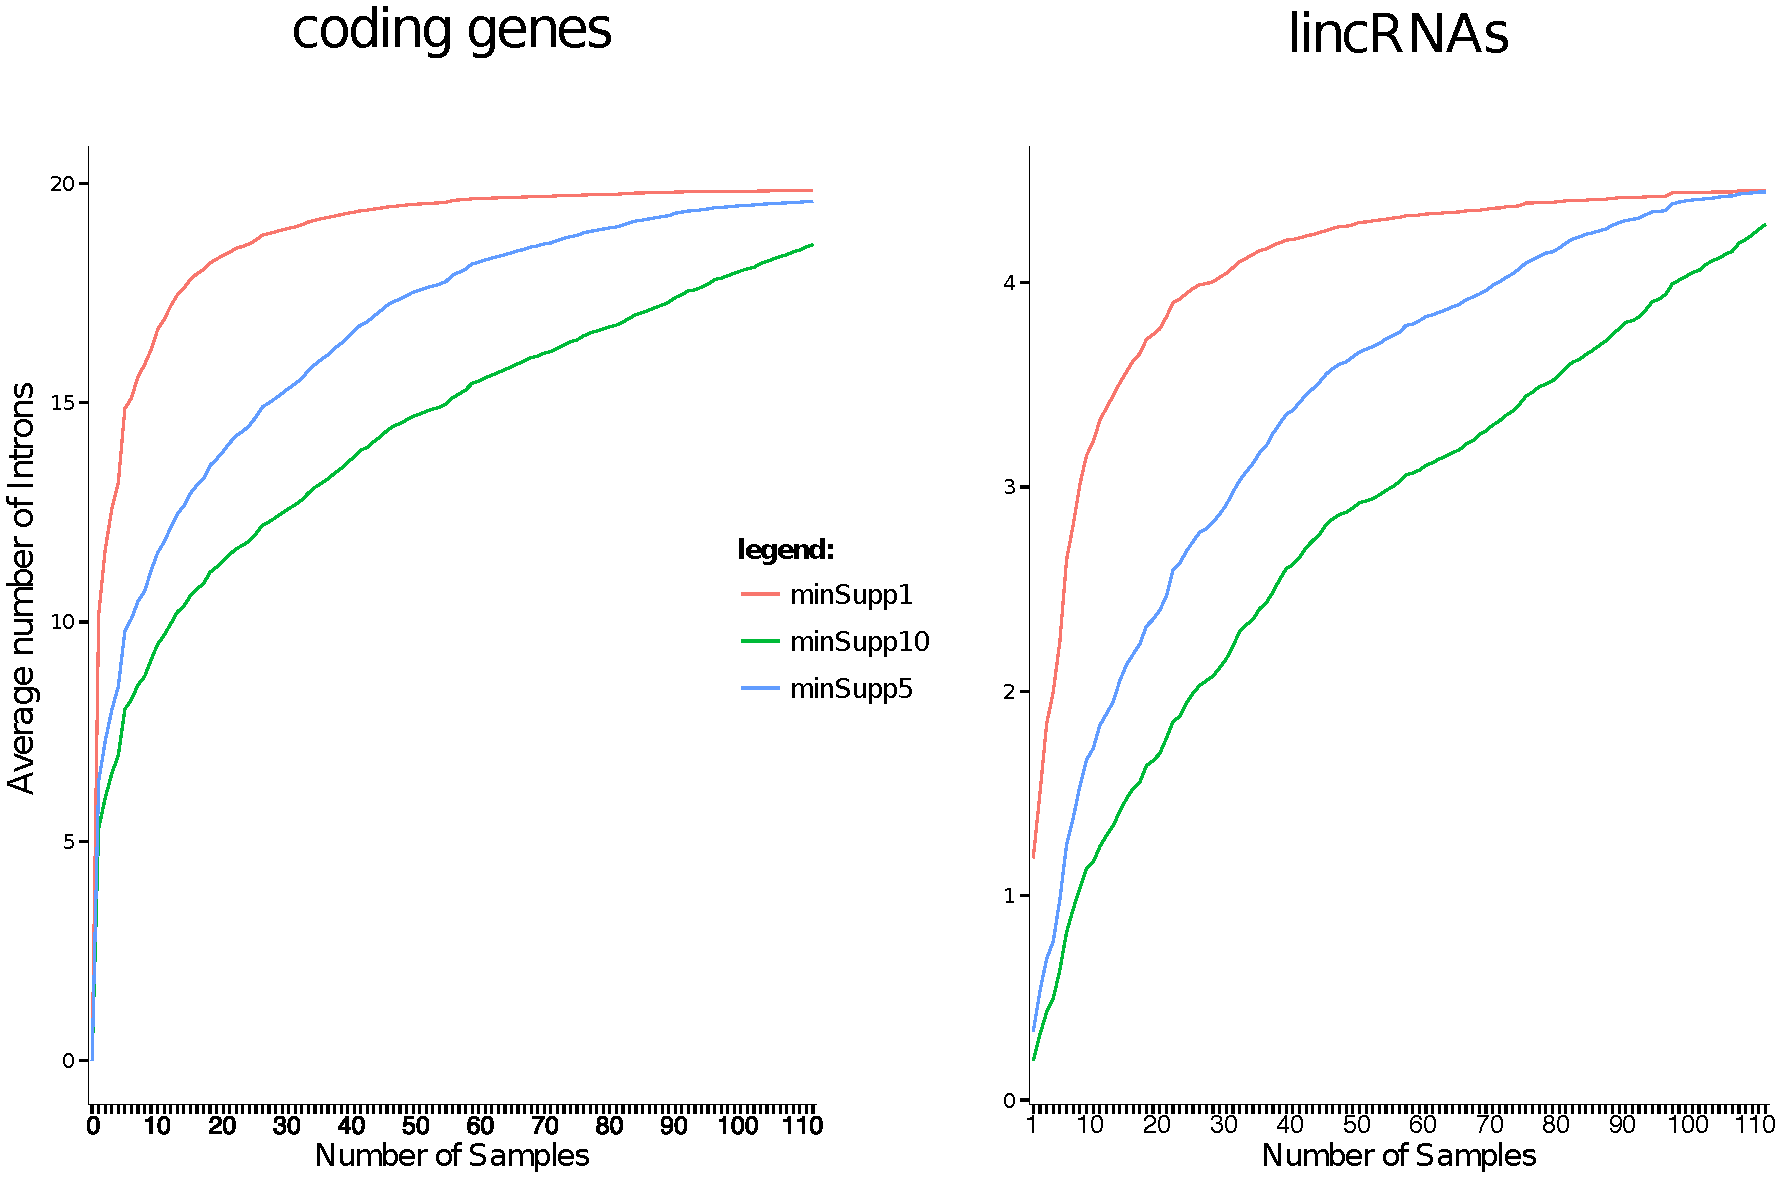
\includegraphics[width=0.8\textwidth]{saturation}
\end{center}
\caption{Saturation curves for the number introns as a function of the 
    number of independent transcriptome samples.}
  \label{fig:saturation} 
\end{figure}

The curves also show that data saturate very slowly, requiring dozens or
even a hundred samples to reach the plateau value. The data shows that the
detected splice junctions are unlikely to be noise: nearly all junctions
seen in at least one sample are reproduced also in 5, and most of them can
be seen in 10 samples, attesting their physical reality. 

\TODO{compare our numbers and ENCODE} \\
Reviewing a part of the ENCODE project, the presence of \textasciitilde{}18 introns in coding genes and \textasciitilde{}4 introns in long intergenic RNAs (lincRNAs) for a minimum read support of 5 was noted, whereas our data yields \textasciitilde{}11 introns per coding gene and \textasciitilde{}2 introns per lincRNA. \\

In Fig.~\ref{fig:compare} we compare our data in more detail with the
GENCODE 19 annotation. For the case of protein-coding loci we tend to miss
some splice junctions at loci that are extremely lowly expressed in the
lymphome transcriptomes. This is not surprising, as rare variants of course
are easier to detect in transcriptomes where they are more highly
expressed; after all, the GENCODE annotation is a composite of vastly
diverse cell types and tissues. It is interesting to note, however, that we
systematically observe more introns at moderate RPKM values even from the
very narrowly defined cell types used here. This attests that large numbers
of well-defined but rare isoforms so far have eluded annotation. 

\begin{figure}[ht]
  \begin{center}
    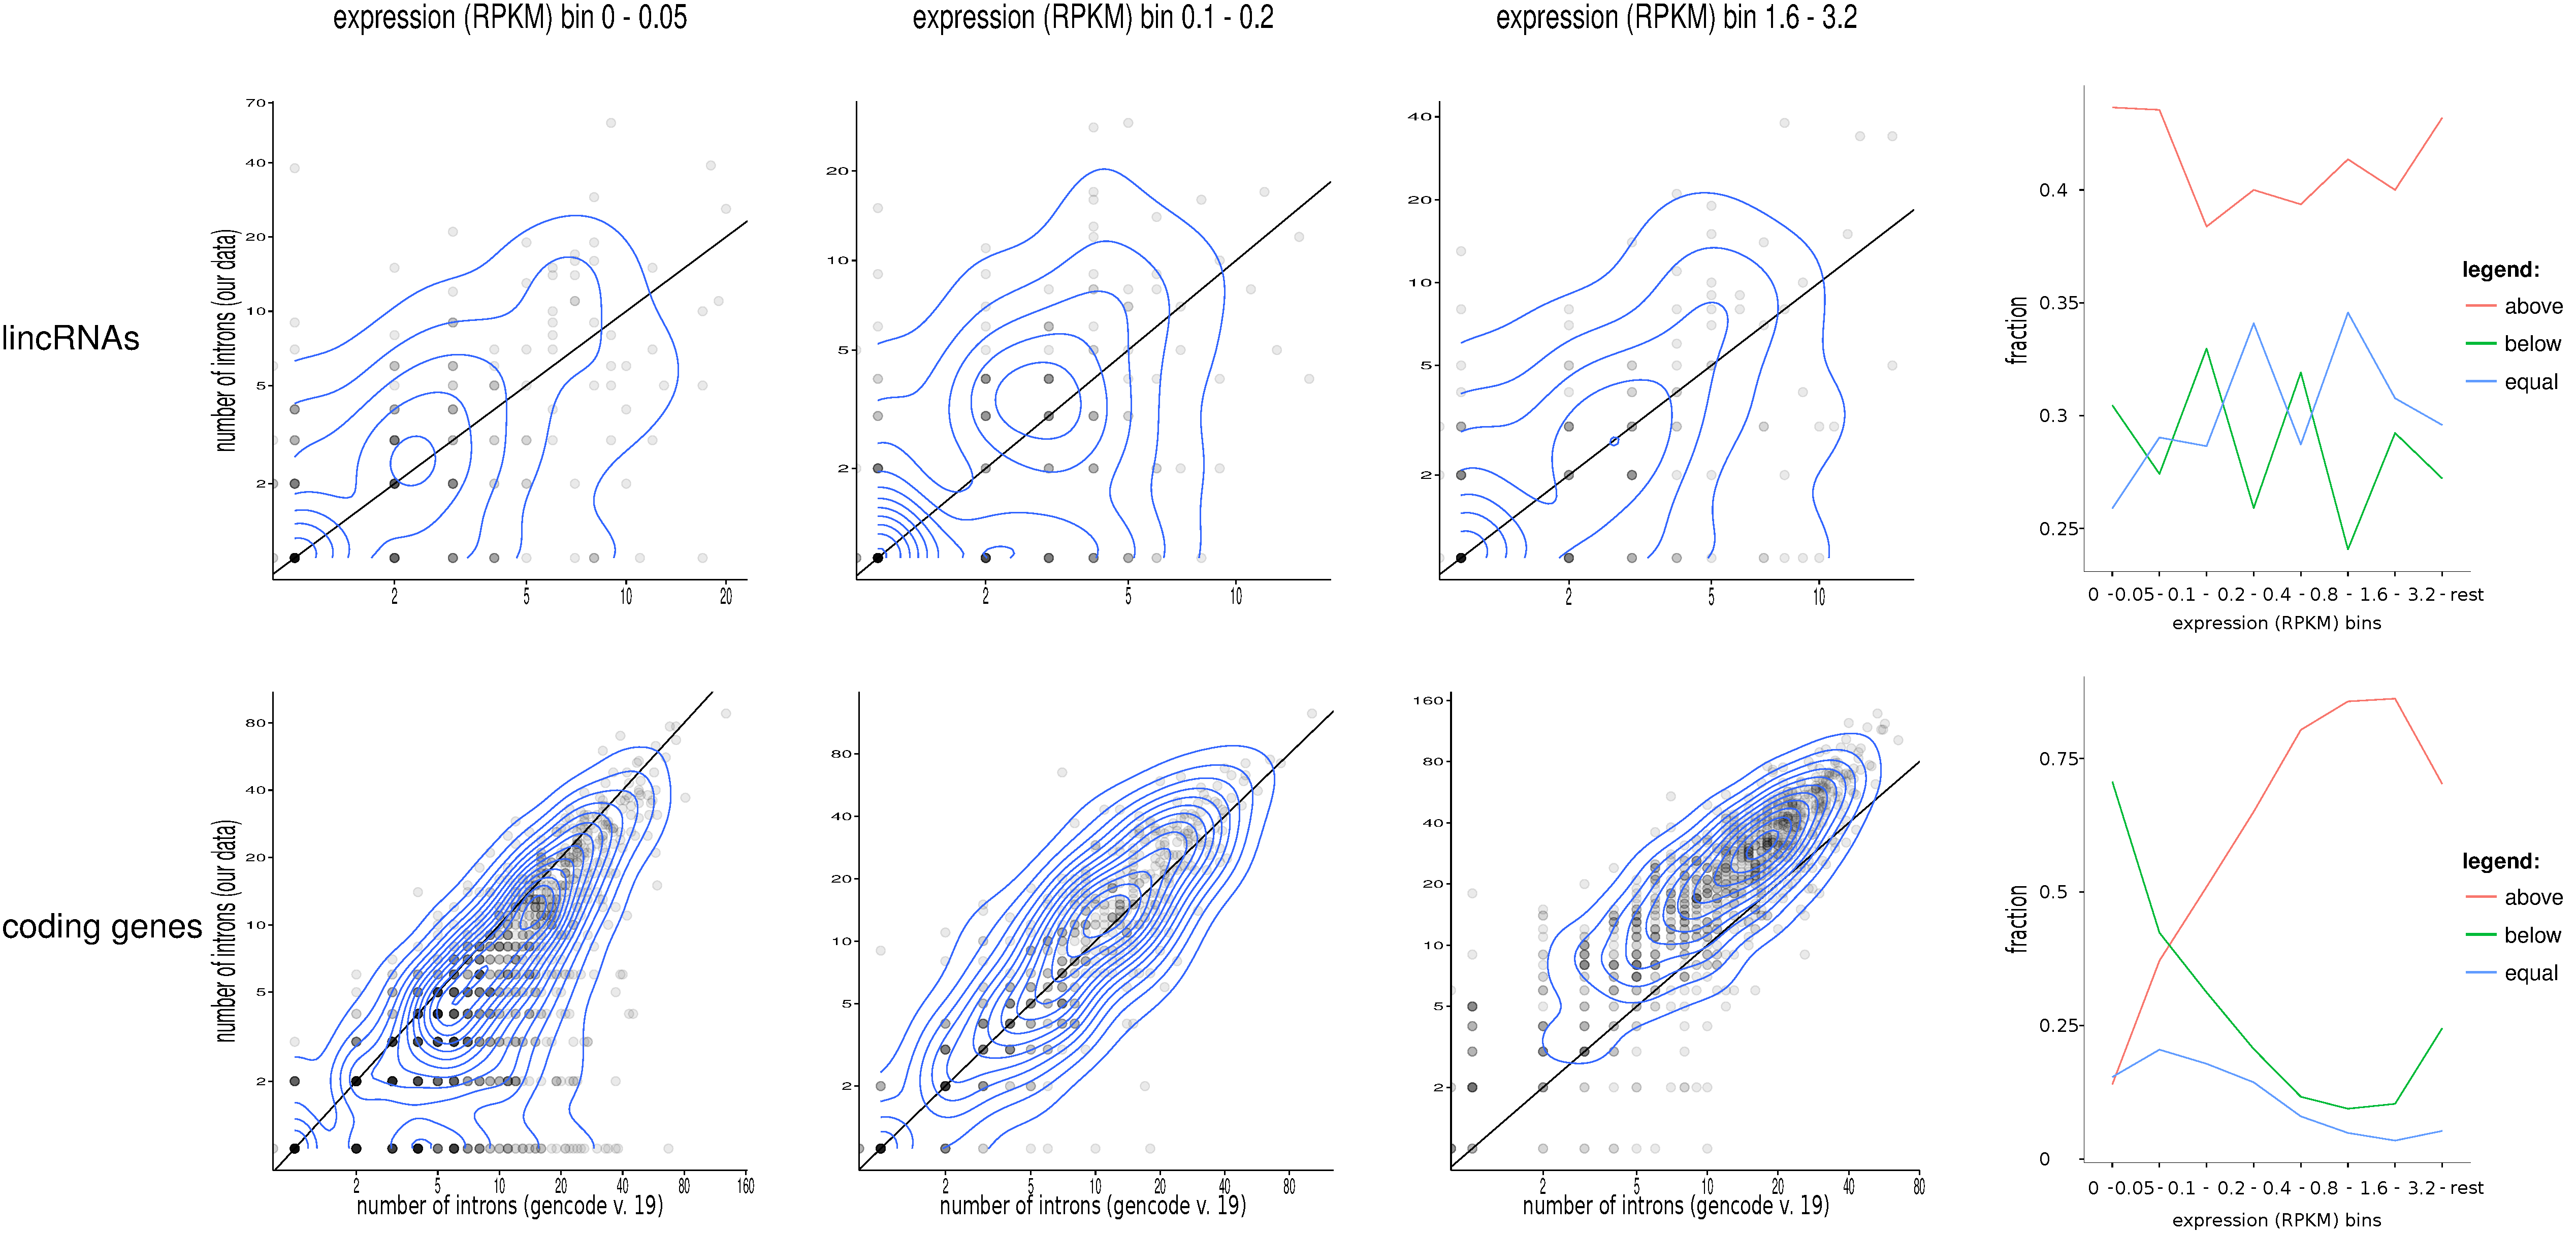
\includegraphics[width=\textwidth]{Fig1}
  \end{center}
  \caption{Scatterplots for different number of expression bins for lincRNAs and coding genes. 
The diagonal is the X=Y line. Points above the line are those genes for that we calculate more introns compared to GENCODE v19.
The right most column shows the fraction of genes being above, below and on the line  in relation to the expression.
While for the coding genes a clear shift of these fractions over the different expression bins is visible, we observe for all expression bins more genes for that we predict more introns compared to the GENCODE v19 annotation.}  
  \label{fig:compare}
\end{figure}

In Fig.~\ref{fig:examples} we show two examples that appear substantially
more complicated in out data in the GENCODE annotation. No functional
annotation is available at present for either locus. As the figure shows,
at least some of the additional exons also appear in EST data tracks
provided by the UCSC genome browser. 

\begin{figure}[t]
\begin{center}
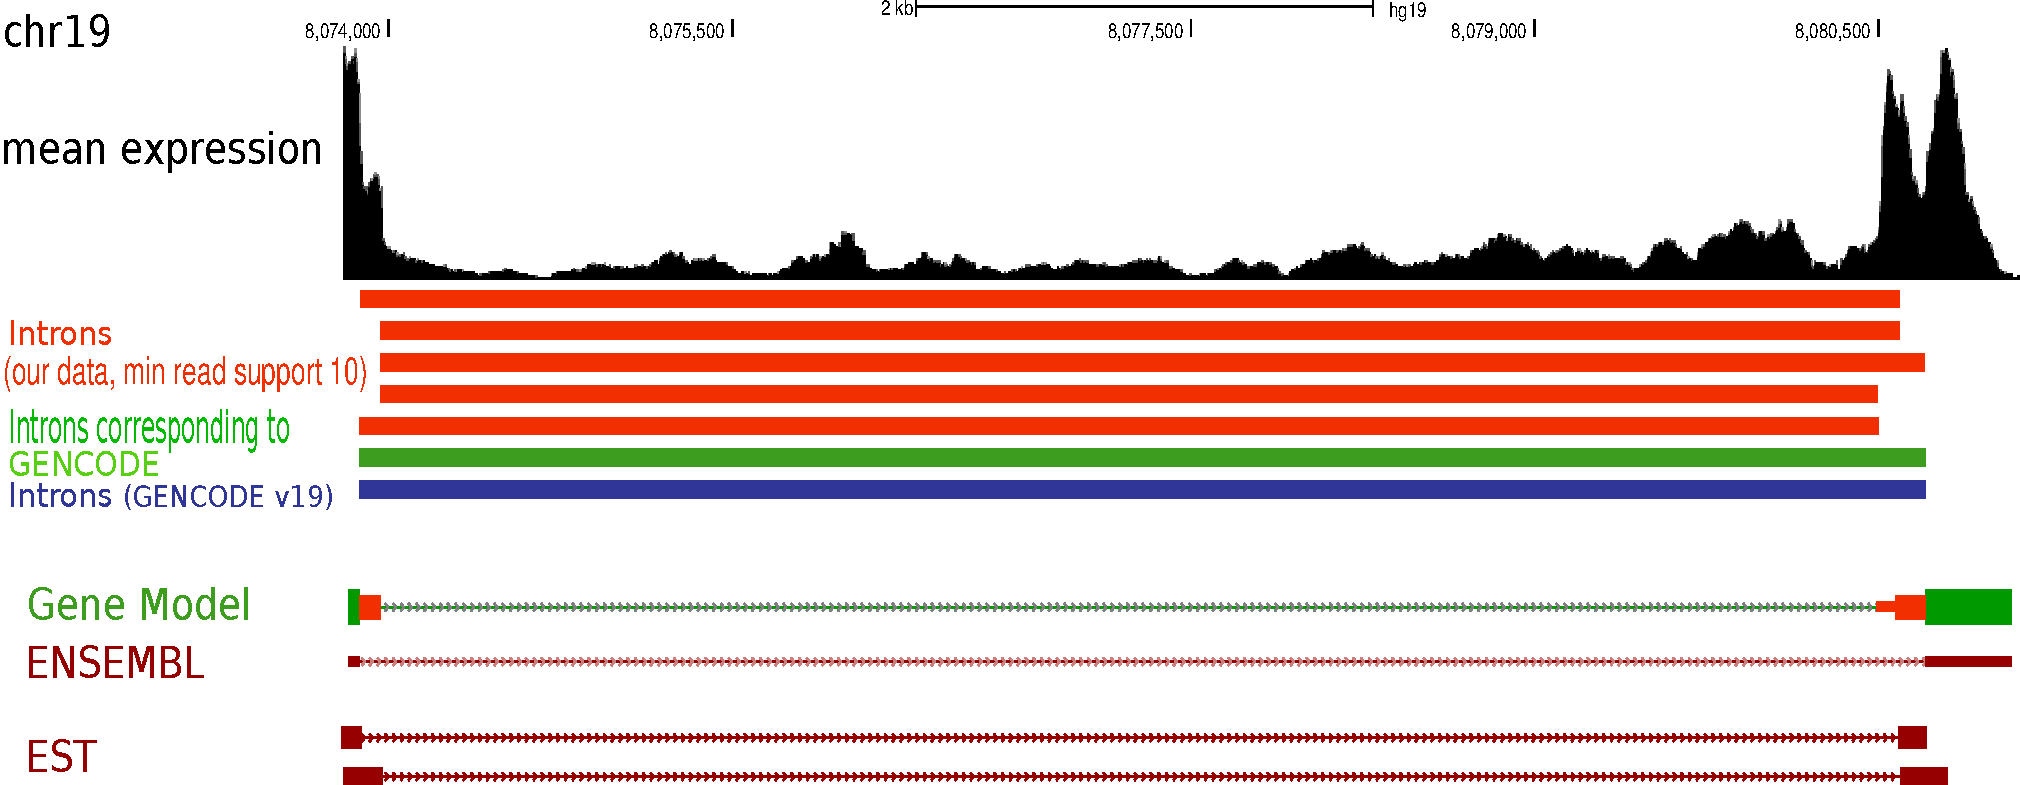
\includegraphics[width=\textwidth]{267939.pdf}\\[1em]
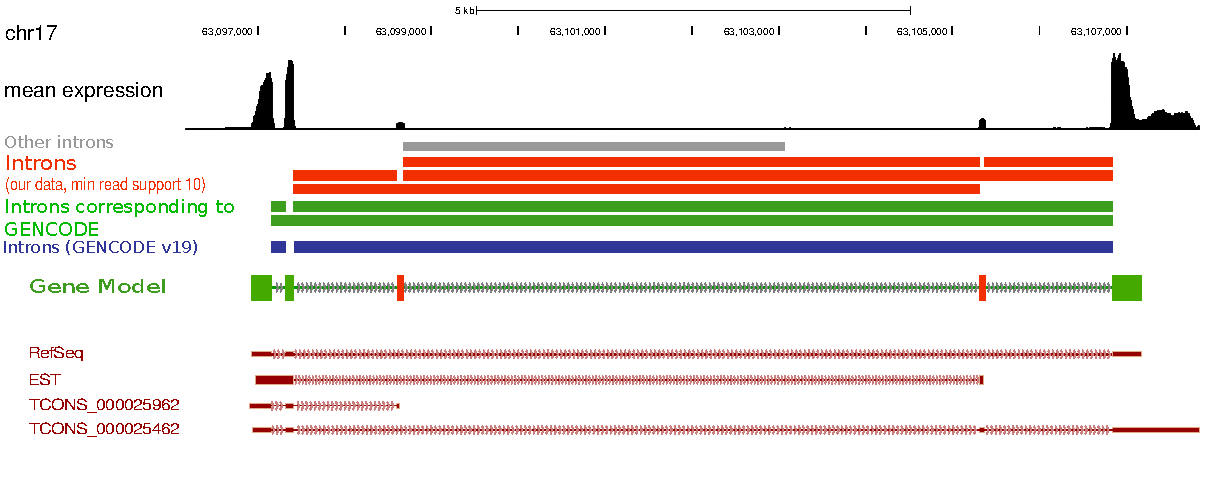
\includegraphics[width=\textwidth]{example.pdf}
\end{center}
\caption{Two examples with previously unannotated splice junctions and
  introns.  (top) In ENSG00000267939 we find 6 introns and two additional
  exons compared to a single intron described in GENCODE v19.  (below) For
  ENSG00000263470 we find 8 introns plus a likely false positive compared
  to 2 introns in GENCODE.}
\label{fig:examples} 
\end{figure}
  
\TODO{more quantitative summary of results!} 

\section{Concluding Remarks} 
	

\section{Materials and Methods}

To understand the sequence structure of the human transcriptome comprehensively, we utilised various annotation datasets to explore the splice junctions already defined there and have a broad overview of the annotation of rare isoforms.
In order to investigate the influence of the dataset size on the complexity of gene structures, we calculated the average number of introns for a series of different dataset sizes.
Therefore, we used RNA-Seq data from 111 lymphoma samples  consisting of the different subtypes BL, FL and DLBCL that was published in the context of the ICGC MMML-Seq project \citep{Richter2012-un}.
First the reads were mapped onto the human reference genome using the splice-aware mapping tool \textit{segemehl} version $0.1.7$ \citep{hoffmann2009,Hoffmann:14a} with split-read option  /texttt{-S} in addition to the default parameters. Then read support for all identified splice junctions, i.e. genomic intervals spanning exon-exon boundaries, were calculated. Since \textit{segemehl} identifies split-reads independently from the annotation, we consider all splice junctions located within genomic coordinates taken from GENCODE version 19 as potential introns. Finally, the average intron number per annotation item was computed using three different minimum read support filters of $1$, $5$ and $10$ respectively.
This procedure was performed using the complete range of all dataset sizes from one sample to all 111 samples (cf. Fig. \ref{fig:saturation}).

Based on the complete data set of all 111 samples we divided the genes according to their normalized mean expressions (RPKM) and counted for all expression bins the number of genes for that we computed more, less or an equal number of introns compared to the annotation using a minimum read support of 10 (Fig. \ref{fig:compare}). 

To analyse the annotation landscape of lncRNAs, the whole transcriptome sequencing data from GENCODE, Ensembl, NONCODE 2016, 
and the dataset from Cabili et. al. were used. GENCODE versions from 7 through 24 were used, as well as Ensembl 54 and 83.
The contents of the datasets are laid out in broadly three categories: the location of the lncRNA gene in the locus, 
the transcripts, and the exon locations within the transcripts. One of the primary aims was to calculate
the number of unique introns in each dataset. 

It is known that, an individual gene can contain multiple transcripts, resulting in the presence of common exons among the transcripts.
 Consequently, a pipeline was created to calculate the unique number of exons present in every gene for every version of each dataset. 
 Each dataset was carefully parsed and filtered to obtain the number of exons present using a simple algorithm. Subsequently the presence of introns were also accounted for.
 
 \paragraph{}
  Ensembl versions 54 and 83 have significant changes in the means of exons, although the medians remain the same(Table 1). The Cabili et. al. dataset and NONCODE document similar means of exons, despite the difference in numbers of genes sampled. Although the number of genes annotated in GENCODE v24 is much greater than in v7, the average presence of exons is less.
 The in house transcriptomic data from different types of cancer (viz. follicular lymphoma, B-cell lymphoma) yielded a lot of lncRNAs. 
 For each of the 5,257 lincRNAs in our dataset, we calculated the transcript count, exonic content of every gene (as in Table 1), if found, in several versions of GENCODE. Although a similarity could be noticed, we computed a number of genes to have higher number of introns than in GENCODE.
  The genes available to us correspond entirely to GENCODE v19.
  On mapping them against v7 and v24, we found that close to 60\% of the genes
 were calculated in v7 and around 95\% in v24(Table 2).

\begin{table}[ht]
\caption{lncRNA genes as catalogued by other consortia} 
\centering
{\tiny
\begin{tabular}[lrrrrrrrr]{p{0.11\textwidth}|p{0.04\textwidth}p{0.08\textwidth}p{0.04\textwidth}p{0.09\textwidth}
p{0.09\textwidth}p{0.05\textwidth}p{0.1\textwidth}p{0.09\textwidth}}
  \hline
 & Genes & Transcripts & Exons & Mean of Exons & Median of Exons & Introns & Mean of Introns & Median of Introns \\ 
   \hline
Ensembl 83 & 9597 & 14038 & 42819 & 3.05 &   3 & 28781 & 2.05 &   2 \\ 
  Ensembl 54 & 15710 & 26799 & 67583 & 2.52 &   3 & 51877 & 1.94 &   2 \\ 
  Cabili 2011 & 8263 & 14353 & 33045 & 2.30 &   2 & 18607 & 1.30 &   1 \\ 
  NONCODE 2016 & 160376 & 233696 & 536111 & 2.29 &   2 & 305771 & 1.31 &   1 \\ 
  GENCODE v7 & 9580 & 14984 & 42060 & 2.81 &   3 & 28998 & 1.94 &   2 \\ 
  GENCODE v24 & 15941 & 28031 & 68457 & 2.44 &   2 & 45016 & 1.61 &   1 \\ 
   \hline
\end{tabular}
}
\end{table}% latex table generated in R 3.3.1 by xtable 1.7-4 package


\begin{table}[ht]
\centering
{\tiny
\begin{tabular}[lrrrrrrrr]{p{0.11\textwidth}|p{0.04\textwidth}p{0.08\textwidth}p{0.04\textwidth}p{0.09\textwidth}
p{0.09\textwidth}p{0.05\textwidth}p{0.1\textwidth}p{0.09\textwidth}}
  \hline
 & Genes & Transcripts & Exons & Mean of Exons & Median of Exons & Introns & Mean of Introns & Median of Introns \\ 
   \hline
v7 & 3296 & 4563 & 12584 & 2.76 & 3 & 8394 & 1.84 & 2\\
  v19 & 5257 & 7487 & 18774 & 2.51 & 2 & 12010 & 1.6 & 1\\
  v24 & 4961 & 7318 & 18685 & 2.55 & 3 & 12202 & 1.67 & 1\\ 
   \hline
\end{tabular}
}
\caption{\update{edited}Transcriptomic data of lncRNA genes from our dataset as reported in GENCODE} 
\end{table}% latex table generated in R 3.3.1 by xtable 1.7-4 package



The GENCODE v7 dataset categorises the lncRNA transcripts as antisense, lincRNA, processed\_transcript and sense\_intronic biotypes. 

The authors reported 9640 lncRNA genes with 15, 512 transcripts and the mean of exons per lncRNA transcript is 2.
Whereas using the same set of genes as can be found in the v7 dataset, 9580 genes with 14984 transcripts were identified in this analysis, although 
the mean of exons per lncRNA transcript was identically computed to be 2.


The current analysis was conducted primarily based on GENCODE datasets from versions 7 through 24. 
The datasets are provided in the standard GTF format. Every dataset classifies a gene with a variety of characteristics, including
the exact locations of genes, their transcripts, and the transcripts contain. As the locations of transcripts overlap in a
gene locus, thus allowing exons to be shared among the transcripts.
Using custom scripts the number of unique exons present in every gene was determined, which also permitted the calculation
of the number of unique introns per gene. Moreover, the number of transcripts for every biotype was also documented.
Furthermore, the mean and median of exons and introns for each dataset was
also computed.


In order to analyse the sequence structure in more details on the UCSC Genome Browser, a batch of genes from the sample dataset 
were carefully identified and selected whose intron content was significanty greater than reported in GENCODE v19. A minimum read support of 10
was further applied to optimise the list.




%%%%%%%%%%%%%%%%%%%%%%%%%%%%%%%%%%%%%%%%%%
\vspace{6pt} 

%%%%%%%%%%%%%%%%%%%%%%%%%%%%%%%%%%%%%%%%%%
%% optional
\supplementary{
The following are available online at www.mdpi.com/link, Figure S1: title, Table
 S1: title, Video S1: title.}

%%%%%%%%%%%%%%%%%%%%%%%%%%%%%%%%%%%%%%%%%%
\acknowledgments{This work was supported in part by the Deutsche
  For\-schungs\-ge\-mein\-schaft grant no. RS is supported by the 
  Deutscher Akademischer Austauschdienst (DAAD).
  }

authorcontributions{PFS designed the study, RS and GD analyzed the data,
  all authors contributed to the interpretation of the results and the
  writing of the manuscript.}

%%%%%%%%%%%%%%%%%%%%%%%%%%%%%%%%%%%%%%%%%%
\conflictofinterests{The authors declare no conflict of interest.}

%%%%%%%%%%%%%%%%%%%%%%%%%%%%%%%%%%%%%%%%%%
%% optional
\abbreviations{The following abbreviations are used in this manuscript:\\

\noindent 
\begin{tabular}{@{}ll}
lncRNA & long non-coding RNA\\
rRNA   & ribosomal RNA
\end{tabular}}

\bibliographystyle{mdpi}
\bibliography{references}

\clearpage 

\end{document}

